\section{Results}

\begin{frame}{Results}
  The main result of this thesis is the representation of the forbidden subgraphs of MUIG as TSG. However, it has been proven that $\mathcal{R}$ is a forbidden subgraph family of TSG. However, we know that TSG $\subseteq$ UUIG.
  \vfill\pause
  \begin{figure}
  \begin{center}
    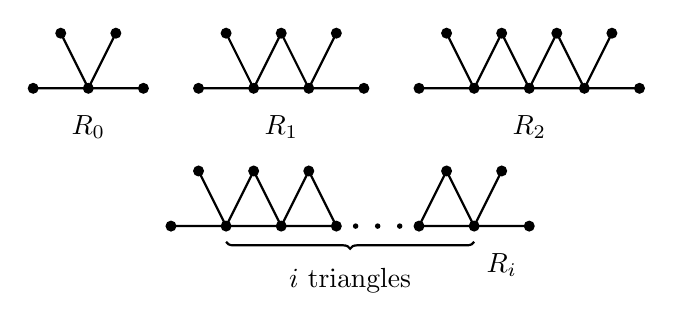
\begin{tikzpicture}[scale=0.7]
  \def\ver{0.1} %size of a vertex
  \def\x{1}

  \def\xa{0.5}
  \def\ya{0}

  \def\xb{4}
  \def\yb{0}

  \def\xc{8}
  \def\yc{0}

  \def\xd{3.5}
  \def\yd{-2.5}


  %graph R_0
  \path[fill] (\xa+0.5,\ya) circle (\ver);
  \path[fill] (\xa+1,\ya+1) circle (\ver);
  \path[fill] (\xa+2,\ya+1) circle (\ver);
  \path[fill] (\xa+2.5,\ya) circle (\ver);
  \path[fill] (\xa+1.5,\ya) circle (\ver);

  \draw[thick] (\xa+0.5,\ya)--(\xa+1.5,\ya)--(\xa+1,\ya+1)
  (\xa+2,\ya+1)--(\xa+1.5,\ya)--(\xa+2.5,\ya);

  \node (1) at (\xa+1.5,\ya-0.7) {$R_0$};

  %graph R_1
  \path[fill] (\xb,\yb) circle (\ver);
  \path[fill] (\xb+1,\yb) circle (\ver);
  \path[fill] (\xb+2,\yb) circle (\ver);
  \path[fill] (\xb+3,\yb) circle (\ver);
  \path[fill] (\xb+0.5,\yb+1) circle (\ver);
  \path[fill] (\xb+1.5,\yb+1) circle (\ver);
  \path[fill] (\xb+2.5,\yb+1) circle (\ver);

  \draw[thick] (\xb,\yb)--(\xb+1,\yb)--(\xb+2,\yb)--(\xb+3,\yb)
  (\xb+0.5,\yb+1)--(\xb+1,\yb)--(\xb+1.5,\yb+1)--(\xb+2,\yb)--(\xb+2.5,\yb+1);

  \node (1) at (\xb+1.5,\yb-0.7) {$R_1$};


  %graph R_2
  \path[fill] (\xc,\yc) circle (\ver);
  \path[fill] (\xc+1,\yc) circle (\ver);
  \path[fill] (\xc+2,\yc) circle (\ver);
  \path[fill] (\xc+3,\yc) circle (\ver);
  \path[fill] (\xc+4,\yc) circle (\ver);
  \path[fill] (\xc+0.5,\yc+1) circle (\ver);
  \path[fill] (\xc+1.5,\yc+1) circle (\ver);
  \path[fill] (\xc+2.5,\yc+1) circle (\ver);
  \path[fill] (\xc+3.5,\yc+1) circle (\ver);

  \draw[thick] (\xc,\yc)--(\xc+1,\yc)--(\xc+2,\yc)--(\xc+3,\yc)--(\xc+4,\yc)
  (\xc+0.5,\yc+1)--(\xc+1,\yc)--(\xc+1.5,\yc+1)--(\xc+2,\yc)--(\xc+2.5,\yc+1)--(\xc+3,\yc)--(\xc+3.5,\yc+1);

  \node (1) at (\xc+2,\yc-0.7) {$R_2$};

  %graph R_i
  \path[fill] (\xd,\yd) circle (\ver);
  \path[fill] (\xd+1,\yd) circle (\ver);
  \path[fill] (\xd+2,\yd) circle (\ver);
  \path[fill] (\xd+3,\yd) circle (\ver);
  \path[fill] (\xd+4.5,\yd) circle (\ver);
  \path[fill] (\xd+5.5,\yd) circle (\ver);
  \path[fill] (\xd+6.5,\yd) circle (\ver);
  \path[fill] (\xd+0.5,\yd+1) circle (\ver);
  \path[fill] (\xd+1.5,\yd+1) circle (\ver);
  \path[fill] (\xd+2.5,\yd+1) circle (\ver);
  \path[fill] (\xd+5,\yd+1) circle (\ver);
  \path[fill] (\xd+6,\yd+1) circle (\ver);

  \fill (\xd+3.35,\yd) circle (\ver/2);
  \fill (\xd+3.75,\yd) circle (\ver/2);
  \fill (\xd+4.15,\yd) circle (\ver/2);

  \draw[thick] (\xd,\yd)--(\xd+3,\yd)
  (\xd+4.5,\yd)--(\xd+6.5,\yd)
  (\xd+0.5,\yd+1)--(\xd+1,\yd)--(\xd+1.5,\yd+1)--(\xd+2,\yd)--(\xd+2.5,\yd+1)--(\xd+3,\yd)
  (\xd+4.5,\yd)--(\xd+5,\yd+1)--(\xd+5.5,\yd)--(\xd+6,\yd+1);

  \draw[thick,decoration={brace,mirror,raise=0.2cm},decorate] (\xd+1,\yd) -- (\xd+5.5,\yd)
  node [pos=0.5,anchor=north,yshift=-0.4cm] {$i$ triangles};

  \node (1) at (\xd+6,\yd-0.7) {$R_i$};

  \end{tikzpicture}
  \end{center}
  \end{figure}
\end{frame}

\begin{frame}{Results}
  \begin{theorem}
    $\mathcal{R}$ is a family of forbidden subgraphs of UUIG.
  \end{theorem}
  \pause
  \begin{proof}
    By induction on $i$.
  \end{proof}

  \vfill
  \begin{figure}
  \begin{center}
    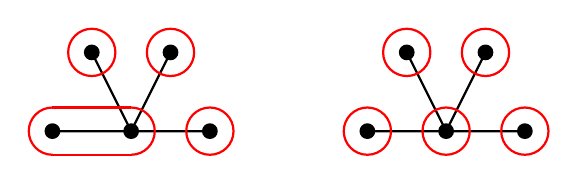
\begin{tikzpicture}[scale=1]
  \def\ver{0.1} %size of a vertex
  \def\x{1}

  \def\xa{0.5}
  \def\ya{0}

  \def\xd{4.5}
  \def\yd{0}


  %graph R_0
  \path[fill] (\xa+0.5,\ya) circle (\ver);
  \path[fill] (\xa+1,\ya+1) circle (\ver);
  \path[fill] (\xa+2,\ya+1) circle (\ver);
  \path[fill] (\xa+2.5,\ya) circle (\ver);
  \path[fill] (\xa+1.5,\ya) circle (\ver);

  \draw[thick] (\xa+0.5,\ya)--(\xa+1.5,\ya)--(\xa+1,\ya+1)
  (\xa+2,\ya+1)--(\xa+1.5,\ya)--(\xa+2.5,\ya);


  \draw[thick,red] (\xa+2,\ya+1+ \ver+0.2) coordinate(a1)  arc (90:450:\ver +0.2) coordinate(a2);

  \draw[thick,red] (\xa+1,\ya+1+ \ver+0.2) coordinate(d1)  arc (90:450:\ver +0.2) coordinate(d2);

  \draw[thick,red] (\xa+2.5,\ya+ \ver+0.2) coordinate(e1)  arc (90:450:\ver +0.2) coordinate(e2);

  \draw[thick,red] (\xa+0.5,\ya+ \ver+0.2) coordinate(b1)  arc (90:270:\ver +0.2) coordinate(b2);
  \draw[thick,red] (\xa+1.5,\ya- \ver-0.2) coordinate(c1)  arc (270:450:\ver +0.2) coordinate(c2);

  % reliate
  \draw[thick,red] (c1) -- (b2) (c2)--(b1);

  %graph R_0
  \path[fill] (\xd+0.5,\yd) circle (\ver);
  \path[fill] (\xd+1,\yd+1) circle (\ver);
  \path[fill] (\xd+2,\yd+1) circle (\ver);
  \path[fill] (\xd+2.5,\yd) circle (\ver);
  \path[fill] (\xd+1.5,\yd) circle (\ver);

  \draw[thick] (\xd+0.5,\yd)--(\xd+1.5,\yd)--(\xd+1,\yd+1)
  (\xd+2,\yd+1)--(\xd+1.5,\yd)--(\xd+2.5,\yd);

  \draw[thick,red] (\xd+2,\yd+1+ \ver+0.2) coordinate(a1)  arc (90:450:\ver +0.2) coordinate(a2);
  \draw[thick,red] (\xd+1,\yd+1+ \ver+0.2) coordinate(d1)  arc (90:450:\ver +0.2) coordinate(d2);
  \draw[thick,red] (\xd+2.5,\yd+ \ver+0.2) coordinate(e1)  arc (90:450:\ver +0.2) coordinate(e2);
  \draw[thick,red] (\xd+1.5,\yd+ \ver+0.2) coordinate(d1)  arc (90:450:\ver +0.2) coordinate(d2);
  \draw[thick,red] (\xd+0.5,\yd+ \ver+0.2) coordinate(e1)  arc (90:450:\ver +0.2) coordinate(e2);

  \end{tikzpicture}
\end{center}\caption{The graph $R_0$.}
  \end{figure}
\end{frame}

\begin{frame}{Results}
  \begin{theorem}
    $\mathcal{R}$ is a family of forbidden subgraphs of UUIG.
  \end{theorem}
  \begin{proof}
    By induction on $i$.
  \end{proof}

  \vfill

  \begin{figure}
  \begin{center}
    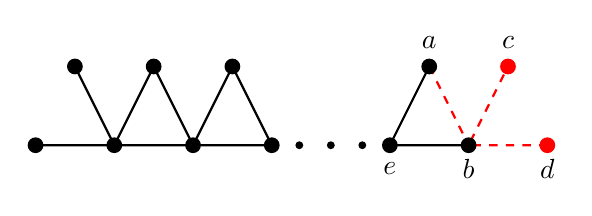
\begin{tikzpicture}[scale=1]
  \def\ver{0.1} %size of a vertex
  \def\x{1}

  \def\xd{0}
  \def\yd{0}

  \draw[thick] (\xd,\yd)--(\xd+3,\yd)
  (\xd+4.5,\yd)--(\xd+5.5,\yd)
  (\xd+0.5,\yd+1)--(\xd+1,\yd)--(\xd+1.5,\yd+1)--(\xd+2,\yd)--(\xd+2.5,\yd+1)--(\xd+3,\yd)
  (\xd+4.5,\yd)--(\xd+5,\yd+1);

  \draw[thick, dashed, color=red] (\xd+6.5,\yd) -- (\xd+5.5,\yd)--(\xd+6,\yd+1) (\xd+5,\yd+1)--(\xd+5.5,\yd);

  %graph R_i
  \path[fill] (\xd,\yd) circle (\ver);
  \path[fill] (\xd+1,\yd) circle (\ver);
  \path[fill] (\xd+2,\yd) circle (\ver);
  \path[fill] (\xd+3,\yd) circle (\ver);
  \path[fill] (\xd+4.5,\yd) circle (\ver);
  \path[fill] (\xd+5.5,\yd) circle (\ver);
  \path[fill, color=red] (\xd+6.5,\yd) circle (\ver);
  \path[fill] (\xd+0.5,\yd+1) circle (\ver);
  \path[fill] (\xd+1.5,\yd+1) circle (\ver);
  \path[fill] (\xd+2.5,\yd+1) circle (\ver);
  \path[fill] (\xd+5,\yd+1) circle (\ver);
  \path[fill, color=red] (\xd+6,\yd+1) circle (\ver);

  \fill (\xd+3.35,\yd) circle (\ver/2);
  \fill (\xd+3.75,\yd) circle (\ver/2);
  \fill (\xd+4.15,\yd) circle (\ver/2);

  \node (1) at (\xd+5.5,\yd-0.3) {$b$};
  \node (2) at (\xd+6.5,\yd-0.3) {$d$};
  \node (2) at (\xd+4.5,\yd-0.3) {$e$};
  \node (4) at (\xd+5,\yd+1+0.3) {$a$};
  \node (3) at (\xd+6,\yd+1+0.3) {$c$};

  \end{tikzpicture}
  \end{center}
  \caption{The graph $R_{i+1}$. You can see that the red edges and vertices are what differ from $R_i$.}\label{fig:ri+1}
  \end{figure}
\end{frame}
